\chapter{RESULTS}
We discuss the results of the topology selection, convergence times, round-trip times, HTTP stress test benchmark results, and video streaming benchmark results in order, comparing the performances of the different network topologies under the two queuing algorithms tested.

\section{Results of clustering and a brief description of the selected topologies}

In general, we have selected topologies of various sizes, some with many loops, and some with structures that are more tree-like. Although this was a sampling from networks with less than 40 nodes, there was still a variety of graph shapes. Figure \ref{fig:groups} shows the clusters formed by the ITZ dataset. Table \ref{tab:choices} describe the key properties of the selected topologies. Together with the baseline topologies described in Section \ref{sec:selection}, the following topologies comprise the set of tested topologies in this study.

\begin{figure}
\centering
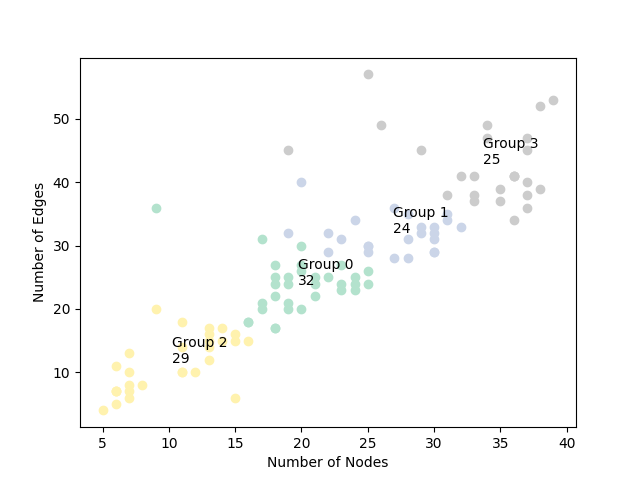
\includegraphics[width=\textwidth]{Figures/clusters.png}
    \caption{133 ITZ topologies as grouped by K-means method based on the number of nodes and number of edges. Numbers in the middle of similarly-colored points indicate the number of topologies in the group.}
    \label{fig:groups}
\end{figure}

\begin{table}[htbp]
    \centering
    \begin{tabular}{ccccc}
    \toprule
        Topology Name & Cluster & \makecell{Number of\\ Nodes} & \makecell{Number of \\Edges} & Location \\
    \midrule
        Savvis (Figure \ref{fig:Savvis}) & 0 & 19 & 20 & USA \\
        Atmnet (Figure \ref{fig:Atmnet})& 0 & 21 & 22 & USA \\
        Ibm (Figure \ref{fig:Ibm})& 0 & 18 & 24 & USA \\
        Agis (Figure \ref{fig:Agis})& 1 & 25 & 30 & USA \\
        WideJpn (Figure \ref{fig:WideJpn})& 1 & 30 & 33 & Japan \\
        Gridnet (Figure \ref{fig:Gridnet})& 2 & 9 & 20 & USA \\
        Nsfnet (Figure \ref{fig:Nsfnet})& 2 & 13 & 15 & USA \\
        Singaren (Figure \ref{fig:Singaren})& 2 & 11 & 10 & Singapore \\
        Janetbackbone (Figure \ref{fig:Janetbackbone})& 3 & 29 & 45 & UK \\
        Canerie (Figure \ref{fig:Canerie})& 3 & 32 & 41 & Canada \\
    \bottomrule
    \end{tabular}
    \caption{10 topologies from the 4 clusters chosen at random with NumPy. Diagrams for these networks are in Appendix I.}
    \label{tab:choices}
\end{table}


\section{Convergence times}
The convergence times between Basic CBQ and Source CBQ were incomparable, as under Basic CBQ, all ping requests were responded to, while in Source CBQ, some number of ping requests failed before the round-trip times stabilized. In Table \ref{tab:convergence}, Basic CBQ has the sum total of the round-trip times before the ping times stabilized below 1 millisecond, and Source CBQ has the number of pings that failed before the ping requests succeded. In all cases, the successful ping requests after the failed requests were under 1 millisecond.

\begin{table}[htbp]
\caption{Convergence times of the tested networks under Basic CBQ and Source CBQ}
\centering
\begin{tabular}{cccc}
\toprule
Cluster & Topology & \multicolumn{2}{c}{Convergence} \\
& & Basic CBQ (ms) & Source CBQ (pings)\\
\midrule
\multirow{3}{*}{0} & Savvis & 16.1 & 12 \\
& Atmnet & 19.2 & 12 \\
& Ibm & 21.1 & 16 \\ \hline
\multirow{2}{*}{1}& Agis & 55.5 & 13 \\
& WideJpn & 37.8 & 17 \\ \hline
\multirow{3}{*}{2}& Gridnet & 11.9 & 9 \\
& Nsfnet & 21.1 & 13 \\
& Singaren & 19.5 & 8 \\ \hline
\multirow{2}{*}{3}& Janetbackbone & 59.6 & 17 \\
& Canerie & 60.5 & 24 \\ \hline
\multirow{2}{*}{Base}& Fat Tree & 21.8 & 10 \\
& Mesh & 11.5 & 11 \\
\bottomrule
\end{tabular}

\label{tab:convergence}
\end{table}

This result shows that Basic CBQ converged faster than Source CBQ in all cases. In all cases, Source CBQ dropped some packets before converging. This will require further investigation to explain the cause. In both algorithms, the smaller topologies (Clusters 2, 0, and Base) converged faster than the larger topologies (Clusters 1, 3). This is expected behavior, since larger networks have more hops between nodes on average, leading to more calls to the SDN controller before converging. Therefore, this demonstrates that the framework properly simulates the real-life networks.

\section{Round-trip times}
The round trip times were similar in both algorithms, as shown in Tables \ref{tab:cbq_pings} and \ref{tab:sbq_pings}. Under both algorithms, smaller networks in general had lower latency, but the difference was not large. Also, across all topologies, Basic CBQ was slightly faster than Source CBQ.

\begin{table}[htbp]
    \caption{Average round-trip times across all clients of the tested networks under Basic CBQ, in milliseconds}
    \centering
    \begin{tabular}{cccccc}
\toprule
Cluster & Topology & Server 1 & Server 2 & Server 3 & Server 4 \\
\midrule
\multirow{3}{*}{0}& Savvis & 0.075 & 0.075 & 0.075 & 0.074 \\
& Atmnet & 0.087 & 0.090 & 0.090 & 0.090 \\
& Ibm & 0.075 & 0.076 & 0.075 & 0.076 \\ \hline
\multirow{2}{*}{1}& Agis & 0.077 & 0.080 & 0.080 & 0.080 \\
& WideJpn & 0.084 & 0.086 & 0.085 & 0.085 \\ \hline
\multirow{3}{*}{2}& Gridnet & 0.068 & 0.069 & 0.069 & 0.069 \\
& Nsfnet & 0.070 & 0.071 & 0.070 & 0.071 \\
& Singaren & 0.062 & 0.064 & 0.063 & 0.063 \\ \hline
\multirow{2}{*}{3}& Janetbackbone & 0.073 & 0.076 & 0.076 & 0.076 \\
& Canerie & 0.082 & 0.084 & 0.085 & 0.084 \\ \hline\multirow{2}{*}{Base}& Fat Tree & 0.063 & 0.064 & 0.063 & 0.063 \\
& Mesh & 0.061 & 0.063 & 0.063 & 0.062 \\

\bottomrule
\end{tabular}

    \label{tab:cbq_pings}
\end{table}

\begin{table}[htbp]
    \caption{Average round-trip times across all clients of the tested networks under Source CBQ, in milliseconds}
    \centering
    \begin{tabular}{lllll}
 & Server 1 & Server 2 & Server 3 & Server 4 \\
Topology &  &  &  &  \\
Fat Tree & 0.066 & 0.066 & 0.066 & 0.067 \\
Mesh & 0.066 & 0.064 & 0.065 & 0.065 \\
Savvis & 0.081 & 0.080 & 0.080 & 0.080 \\
Atmnet & 0.094 & 0.093 & 0.095 & 0.094 \\
Ibm & 0.078 & 0.078 & 0.078 & 0.078 \\
Agis & 0.081 & 0.081 & 0.081 & 0.080 \\
WideJpn & 0.087 & 0.086 & 0.086 & 0.086 \\
Gridnet & 0.073 & 0.072 & 0.071 & 0.071 \\
Nsfnet & 0.074 & 0.072 & 0.072 & 0.074 \\
Singaren & 0.068 & 0.067 & 0.068 & 0.067 \\
Janetbackbone & 0.082 & 0.080 & 0.080 & 0.080 \\
Canerie & 0.083 & 0.084 & 0.084 & 0.083 \\
\end{tabular}

    \label{tab:sbq_pings}
\end{table}

While smaller topologies in clusters 0, 2 and the base topologies performed better than clusters 3 in both algorithms in this benchmark, Atmnet, which is the worst performing topology in this benchmark, is not the largest topology among the sampled topologies. This suggests that the shape and structure of the underlying graph also matters in round-trip time performance. In this case, Atmnet is a network consisting of two large rings. This may be the reason for the worse performance: the STP protocol chooses a spanning tree through the network, and in the specific case of Atmnet, the chosen is bound to be large due to the shape of the network.

\section{HTTP file transfer traffic performance}

HTTP file transfer traffic as generated by the \textsc{hey} program was the best-effort traffic in this experiment. We used the following KPIs: Number of successful transfers, number of failures, Total bytes transferred and transfer rate. Tables \ref{tab:cbq_http} and \ref{tab:sbq_http} show the average results for Basic CBQ and Source CBQ, respectively.

\begin{table}[htbp]
    \caption{Average HTTP file transfer performance across all clients of the tested networks under Basic CBQ}
    \centering
    \begin{tabular}{cccccc}
\toprule
Cluster & Topology & \thead{Total Transferred\\Data (bytes)} & \thead{Transfer Rate\\(kB/s)} & Success & Failure \\
\midrule
\multirow{3}{*}{0}& Savvis & \num{960048736} & 3145.488 & 2721.21 & 0.02 \\
& Atmnet & \num{1365445427} & 4416.213 & 2327.46 & 0.00 \\
& Ibm & \num{1486840762} & 4801.515 & 1532.22 & 0.13 \\ \hline
\multirow{2}{*}{1}& Agis & \num{1199376942} & 3840.219 & 846.62 & 0.02 \\
& WideJpn & \num{973259047} & 3146.767 & 610.73 & 0.00 \\ \hline
\multirow{3}{*}{2}& Gridnet & \num{2071584230} & 6628.799 & 1735.27 & 0.00 \\
& Nsfnet & \num{1582198537} & 5058.813 & 1881.84 & 0.00 \\
& Singaren & \num{3366646614} & 10521.097 & 437.91 & 1.31 \\ \hline
\multirow{2}{*}{3}& Janetbackbone & \num{733299798} & 2382.739 & 598.05 & 0.05 \\
& Canerie & \num{950662835} & 3113.366 & 2631.67 & 0.05 \\ \hline
\multirow{2}{*}{Base}& Mesh & \num{6042224106} & 18326.877 & 484.09 & 7.02 \\
& Fat Tree & \num{2449880430} & 7530.391 & 454.69 & 0.62 \\
\bottomrule
\end{tabular}

    \label{tab:cbq_http}
\end{table}

\begin{table}[htbp]
    \caption{Average HTTP file transfer performance across all clients of the tested networks under Source CBQ}
    \centering
    \begin{tabular}{cccccc}
\toprule
Cluster & Topology & \makecell{Total Transferred\\Data (bytes)} & \makecell{Transfer Rate\\(KB/s)} & Success & Failure \\
\midrule
\multirow{3}{*}{0} & Savvis & \num{1552970252} & 4644.084 & 201.92 & 13.50 \\
& Atmnet & \num{1231539541} & 3655.377 & 191.81 & 16.19 \\
& Ibm & \num{1400247275} & 4185.324 & 219.19 & 9.04 \\ \hline
\multirow{2}{*}{1}& Agis & \num{910867519} & 2710.260 & 80.62 & 87.73 \\
& WideJpn & \num{872243200} & 2586.718 & 123.75 & 18.84 \\ \hline
\multirow{3}{*}{2} & Gridnet & \num{2851570329} & 8716.683 & 164.70 & 8.86 \\
& Nsfnet & \num{2117366616} & 6471.987 & 144.35 & 7.13 \\
& Singaren & \num{4498343146} & 13571.177 & 238.70 & 11.49 \\ \hline
\multirow{2}{*}{3}& Janetbackbone & \num{862200493} & 2574.689 & 177.73 & 15.54 \\
& Canerie & \num{753304312} & 2241.503 & 172.28 & 20.67 \\ \hline
\multirow{2}{*}{Base}& Fat Tree & \num{4335677792} & 13071.211 & 234.28 & 13.43 \\
& Mesh & \num{3600709838} & 11137.290 & 179.62 & 9.88 \\
\bottomrule
\end{tabular}

    \label{tab:sbq_http}
\end{table}

Clearly, the Basic CBQ outperformed Source CBQ in terms of reliability, since there were little to no clients that failed to receive data. Under Source CBQ, the number of failed requests was generally higher in larger topologies, with the Agis topology being an outlier. However, in terms of average transfer rate, some topologies performed better under Source CBQ instead of Basic CBQ. A comparison is provided in Table \ref{tab:trasfer_rate_comparison}.

\begin{table}[htbp]
    \caption{Comparison of average trasfer rates of the tested networks under Class CBQ and Source CBQ}
    \centering
    \begin{tabular}{cccc}
\toprule
\multirow{2}{*}{Cluster} & \multirow{2}{*}{Topology} & \multicolumn{2}{c}{Transfer Rate (kB/s)} \\
& & Basic CBQ & Source CBQ \\
\midrule
\multirow{3}{*}{0} & Savvis & \num{3145.488} & \num{4644.084} \\
& Atmnet & \num{4416.213} & \num{3655.377} \\
& Ibm & \num{4801.515} & \num{4185.324} \\ \hline
\multirow{2}{*}{1} & Agis & \num{3840.219} & \num{2170.260} \\
& WideJpn & \num{3146.767} & \num{2586.718} \\ \hline
\multirow{3}{*}{2} & Gridnet & \num{6628.799} & \num{8716.683} \\
& Nsfnet & \num{5058.813} & \num{6471.987} \\
& Singaren & \num{10521.097} & \num{13571.177} \\ \hline
\multirow{2}{*}{3} & Janetbackbone & \num{2382.739} & \num{2574.689} \\
& Canerie & \num{3113.366} & \num{2241.503} \\ \hline
\multirow{2}{*}{Base} & Mesh & \num{18326.877} & \num{13071.211} \\ 
& Fat Tree & \num{7530.391} & \num{11137.290}\\
\bottomrule
\end{tabular}


    \label{tab:trasfer_rate_comparison}
\end{table}

This is likely because in the instances where Source CBQ performed better than Basic CBQ, some clients had requested for larger files, and those requests were served better than the requests for smaller files under Source CBQ. We notice also that the number of successful requests in Basic CBQ are much higher than the same in Source CBQ across all topologies. This is likely because in Basic CBQ, the requests for smaller files were served better than the requests for larger files.

We also note that for all Cluster 2 topologies, as well as the similarly-sized Fat-tree topology, Source CBQ had higher transfer rates results. These topologies are common in the fact that they have tree-like shapes with low tree height; that is, the farthest edge nodes are not so far in terms of the number of hops from the root node as described in Section \ref{sec:topo_config}.

However, we also observe that Savvis and Atmnet, which are two topologies similar both in shape and size, had opposite behavior in terms of which algorithm had better transfer rate. This suggests that the volume and type of traffic from the hosts closer to the root node may affect the results of the simulation, as indicates earlier.

\section{Video traffic performance}
In this experiment, VLC traffic was considered as the high--priority traffic. To measure VLC traffic performance, we took note of the following Key Performance Indicators (KPIs): the total demux bytes read, the demux bitrate, the average number of successful streams and failed streams. In Basic CBQ, video traffic performance was consistent throughout all topologies (Table \ref{tab:cbq_vlc}, with no disconnections or failed connections. However, In Source CBQ, topologies in the clusters with larger networks suffered disconnections, therefore the total demux bytes read and the bitrate was also affected (Table \ref{tab:sbq_vlc}. This can be attributed to the fact that in Source CBQ, in each of the queues, there is neither separation nor priority among the different traffic types.

\begin{table}[htbp]
    \caption{Average video streaming performance across all clients of the tested networks under Basic CBQ}
    \centering
    \begin{tabular}{ccccccc}
\toprule
\thead{Cluster} & \thead{Topology} & \thead{Demux Bytes\\Read (Bytes)} & \thead{Average Bitrate\\(bps)} & \thead{Success} & \thead{Disconnected} & \thead{Failed} \\
\midrule
\multirow{3}{*}{0} &Savvis & \num{46536544} & \num{1201.371} & 48.00 & 0.00 & 0.00 \\
&Atmnet & \num{46552912} & \num{1202.587} & 48.00 & 0.00 & 0.00 \\
&Ibm & \num{46602219} & \num{1208.467}& 48.00 & 0.00 & 0.00 \\ \hline
\multirow{2}{*}{1}&Agis & \num{46545751} & \num{1201.322}& 48.00 & 0.00 & 0.00 \\
&WideJpn & \num{46534391} & \num{1200.953}& 48.00 & 0.00 & 0.00 \\ \hline
\multirow{3}{*}{2}&Gridnet & \num{46556621} & \num{1203.631}& 48.00 & 0.00 & 0.00 \\
&Nsfnet & \num{46556302} & \num{1203.572}& 48.00 & 0.00 & 0.00 \\
&Singaren & \num{46082974} & \num{1222.016}& 48.00 & 0.00 & 0.00 \\ \hline
\multirow{2}{*}{3}&Janetbackbone & \num{46535836} & \num{1200.260}& 48.00 & 0.00 & 0.00 \\
&Canerie & \num{46548273} & \num{1200.553}& 48.00 & 0.00 & 0.00 \\ \hline
\multirow{2}{*}{Base}&Fat Tree & \num{46139946} & \num{1218.847} & 48.00 & 0.00 & 0.00 \\
&Mesh & \num{46629398} & \num{1207.949}& 48.00 & 0.00 & 0.00 \\

\bottomrule
\end{tabular}

    \label{tab:cbq_vlc}
\end{table}

\begin{table}[htbp]
    \caption{Average video steraming performance across all clients of the tested networks under Source CBQ}
    \centering
    \begin{tabular}{ccccccc}
\toprule
\thead{Cluster} & \thead{Topology} & \thead{Demux Bytes\\Read (Bytes)} & \thead{Average Bitrate\\(bps)} & \thead{Success} & \thead{Disconnected} & \thead{Failed} \\
\midrule
\multirow{3}{*}{0} & Savvis & \num{25409794} & 579.678 & 26.90 & 16.00 & 5.10 \\
& Atmnet & \num{22202970} & 493.266 & 23.03 & 17.00 & 7.97 \\
& Ibm & \num{29750840} & 685.056 & 30.77 & 14.33 & 2.90 \\ \hline
\multirow{2}{*}{1}& Agis & \num{14259713} & 295.468 & 12.47 & 14.80 & 20.73 \\
& WideJpn & \num{21871343} & 509.422 & 23.03 & 20.80 & 4.17 \\ \hline
\multirow{3}{*}{2}& Gridnet & \num{38443307} & 1019.329 & 48.00 & 0.00 & 0.00 \\
& Nsfnet & \num{35100719} & 936.028 & 47.97 & 0.03 & 0.00 \\
& Singaren & \num{40815092} & 1119.248 & 48.00 & 0.00 & 0.00 \\ \hline
\multirow{2}{*}{3}& Janetbackbone & \num{21279821} & 449.191 & 18.53 & 22.67 & 6.80 \\
& Canerie & \num{19737077} & 434.172 & 18.07 & 23.57 & 6.37 \\ \hline
\multirow{2}{*}{Base}& Fat Tree & \num{39351946} & 1079.992 & 46.30 & 1.17 & 0.53 \\
& Mesh & \num{39590074} & 1059.317 & 48.00 & 0.00 & 0.00 \\
\bottomrule
\end{tabular}

    \label{tab:sbq_vlc}
\end{table}

Based on this result, we can conclude that Basic CBQ is better at providing QoS guarantees for video traffic than Source CBQ. In Basic CBQ, Clusters 0 and 2, which is composed of the smaller topologies, universally performed better than Clusters 1 and 3, which are the larger topologies. This shows that unlike the HTTP traffic benchmark, the video streaming results are more directly affected by topology size (number of nodes and edges), in cases where the performance guarantee is not consistent.

\section{Summary of Results}

Table \ref{tab:summary} shows the summary of the Key Performance Indicators (KPIs) of this experiment, which are the round-trip times, HTTP Transfer rates, and Video Demux Bitrate. In all clusters, as well as the baseline topologies, Basic CBQ performed slightly better than Source CBQ in round-trip times, but the difference was minimal. In transfer rate, Source CBQ was better than Basic CBQ in Cluster 2, which contained the smallest topologies. Source CBQ was almost equal in Cluster 0, and worse in the larger topologies in Cluster 1 and 3 than Basic CBQ. For demux bitrate, Basic CBQ performed better than Source CBQ across all topologies, but the difference became more significant in Clusters 1 and 3, which represent the larger topologies. It is also important to note that the fat-tree topology, which is similar in size to Cluster 2, had similar results to the average of Cluster 2 topologies. The smallest mesh topology, with 5 nodes only, outperformed all other, larger topologies, which further confirms that the framework exhibited results within expectations.

\begin{table}[htbp]
    \caption{Average of key performance indicators by cluster, for Basic CBQ and Source CBQ}
    \centering
    \begin{tabular}{ccccccc}
    \toprule
    \multirow{2}{*}{Cluster} & \multicolumn{2}{c}{\makecell{Round Trip Times\\(ms)}} & \multicolumn{2}{c}{\makecell{Transfer Rate\\(KB/s)}} & \multicolumn{2}{c}{\makecell{Demux Bitrate\\(bps)}} \\
    & Basic & Source & Basic & Source & Basic & Source \\  \midrule
    0 & 0.080 & 0.084 & 4121.072 & 4161.595 & 1204.142 & 586.000 \\ 
    1 & 0.082 & 0.084 & 3493.493 & 2378.489 & 1201.138 & 402.445 \\ 
    2 & 0.067 & 0.071 & 7402.903 & 9586.616 & 1209.740 & 1024.868 \\ 
    3 & 0.080 & 0.082 & 2748.053 & 2408.096 & 1200.407 & 441.682 \\ 
    Mesh & 0.062 & 0.066 & 18326.877 & 13071.211 & 1207.949 & 1079.992 \\ 
    Fat-tree & 0.063 & 0.065 & 7530.391 & 11137.290 & 1218.847 & 1059.317 \\ \bottomrule
\end{tabular}
    \label{tab:summary}
\end{table}

These results show a more dramatic difference between Basic CBQ and Source CBQ than the experiments by Regencia and Yu \cite{yang_introducing_2022}. In that experiment, Basic CBQ and Source CBQ performed similarly across the tree topologies of various sizes. While a direct comparison between the results of the experiments in Regencia and Yu is not possible because of the differences in the controller and the test machines, relative performance of Basic CBQ was much better in this experiment than Source CBQ. This suggests that in a variety of topologies, Basic CBQ performed much better than Source CBQ. However, the results for the Fat-tree (fanout 3, 2 layers) topology of this experiment exhibited a bigger difference between Basic CBQ and Source CBQ than the difference exhibited by the previous experiment. This suggests a need for further validation of the results of this study.

We also note that the Mesh topology, which is the smallest topology consisting of only 5 nodes, performed significantly better than the other nodes. This is likely due to two factors: one, simply that the topology is the smallest, and smaller topologies perform generally better, and two, that since the ideal Mesh topology had \textit{all} possible links to start with, the Spanning Tree Protocol was able to select the optimum spanning tree, increasing the performance. This suggests that one variable that can be further changed is the protocol for resolving loops in the network.

Finally, we note some commonalities in the topologies. The topologies most similar to the Fat Tree were the topologies in Cluster 2, which had tree or tree-like structure. Therefore, the KPIs also exhibited similar results. Cluster 1 and Cluster 3 topologies were similarly sized in terms of the number of nodes, but Cluster 3 had more edges, and therefore were in diffrent clusters. This is likely why Cluster 1 and 3 topologies had similar KPIs, with Cluster 1 topologies beating Cluster 3 in some KPIs (esp. in Basic CBQ) adnd Cluster 3 beating Cluster 1 in other KPIs (esp. in Source CBQ). This result points to a need for more stringent studies on which topology factors affect the performance of the QoS algorithms.
